\section{Data processing and classification}
\label{sec:methodology}

The classification study consists of a reconstruction of the source
experiment, which uses its two original channels, and an extension to the six
responses of Table~\ref{tab:channels} and to a third network arm with
multi-rate pooling. Both use the same simulated passages, data partition,
measurement noise, and initialization seeds, so their differences are not
affected by resampling of the dataset.

\subsection{Data partition, measurement noise, and preprocessing}
\label{sec:preprocessing}

The passages of each scenario are split into 80 training, 20 validation, and
100 test passages, as in the source. The allocation is a single random
permutation of the passage indices (PCG64 generator, seed 2025080901), applied
identically to all scenarios and all configurations; the training, validation,
and test sets therefore contain 800, 200, and 1,000 passages. Each scenario is
one fixed structural configuration, so this split measures the recognition of
known configurations under new operational conditions, not the generalization
to unseen damage states.

Measurement noise follows Eq.~(2) of the source~\cite{fernandes2025early}:
\begin{equation}
    x^{\mathrm{noisy}}_i=x_i+0.05\,\sigma(x)\,\epsilon_i,
    \qquad \epsilon_i\sim\mathcal{N}(0,1),
    \label{eq:noise}
\end{equation}
where $\sigma(x)$ is the standard deviation of the clean signal $x$ of one
passage and channel. One noise realization is generated for each scenario,
passage, and channel and is shared by all representations and networks. Each
channel is then min--max normalized,
\begin{equation}
    \tilde{x}_i=\frac{x_i-x_{\min}}{x_{\max}-x_{\min}},
\end{equation}
with $x_{\min}$ and $x_{\max}$ computed on the training set only and applied
without clipping to the validation and test sets. RAW inputs keep all 5,830
normalized samples. PAA inputs~\cite{keogh2001dimensionality} replace each
block of ten consecutive samples by its mean, giving 583 values per channel, the
segment length selected in the source study.

\subsection{CNN architectures}
\label{sec:architectures}

RAW-CNN and PAA-CNN reproduce the source architecture
(Fig.~\ref{fig:f25_architecture}): one to five one-dimensional convolutional
layers without padding and with ReLU activation, each optionally followed by
max pooling of size two, a flatten layer, a dense ReLU layer, and a ten-class
output layer. PAA-MR (PAA with multi-rate pooling) replaces the flatten layer
by adaptive max pooling at resolutions of 1, 2, and 4 bins, inspired by the
multi-rate sampling of N-HiTS~\cite{challu2023nhits}, and concatenates the seven
pooled values of each feature map before the dense layer. Flattening already
preserves the position of the features along the bridge, so multi-rate pooling
is an alternative aggregation rather than a means of adding positional
information. It also reduces the width of the dense-layer input and the number
of parameters, so an accuracy difference between the arms cannot be attributed
to a single mechanism.

\begin{figure}[htbp]
\centering
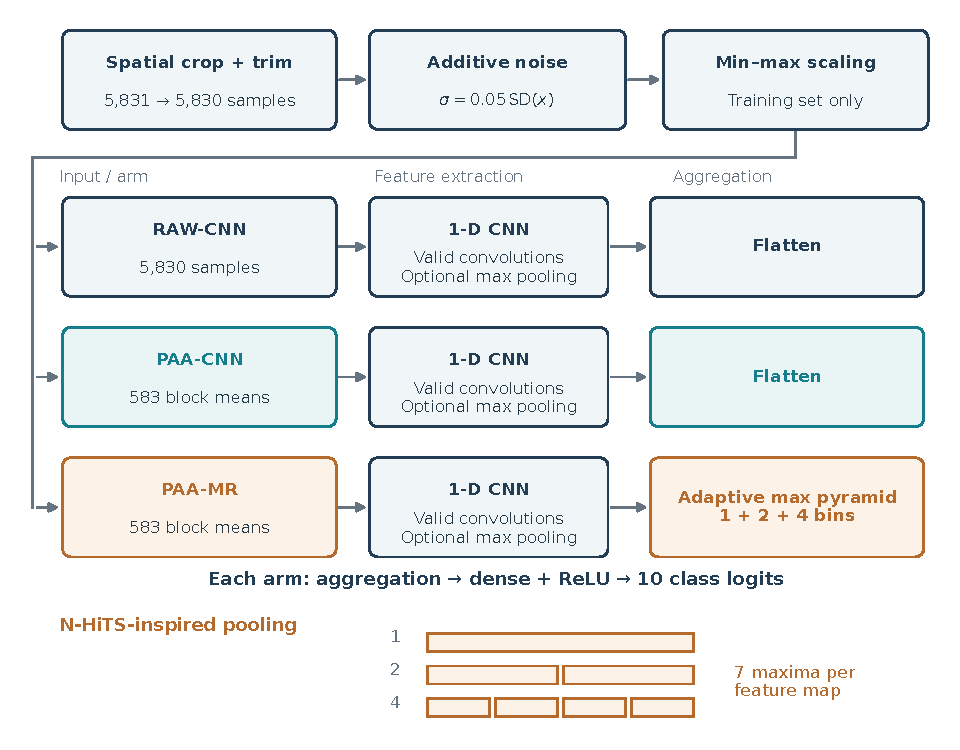
\includegraphics[width=0.92\textwidth]{f25_architecture.pdf}
\caption{Preprocessing and network arms. RAW-CNN and PAA-CNN flatten the last
feature maps; PAA-MR replaces flattening with adaptive max pooling at 1, 2, and
4 bins, giving seven values per feature map. All arms end in a dense ReLU layer
and ten class outputs.}
\label{fig:f25_architecture}
\end{figure}

\subsection{Hyperparameter optimization and training}
\label{sec:hpo}

Hyperparameters are tuned by Bayesian optimization with the tree-structured
Parzen estimator~\cite{bergstra2011algorithms} implemented in
Optuna~\cite{akiba2019optuna}. As in the source, each optimization comprises
100 proposals, and each proposal is trained five times, here with fixed seeds;
the objective is the mean validation accuracy of the five runs. The search space
is that of the source: one to five convolutional layers, 32--128 filters in
steps of 16, kernel sizes of 2--5, optional max pooling after each layer, 16--64
dense units in steps of 16, batch sizes of 8--48 in steps of 8, and a learning
rate between $10^{-5}$ and $10^{-2}$, sampled on a logarithmic scale.

The networks are trained with the Adam optimizer~\cite{kingma2015adam} and the
cross-entropy loss. The learning rate is halved after 30 epochs without
improvement of the validation loss, down to $10^{-6}$, and training stops after
50 epochs without improvement or at 1,000 epochs; these settings follow the
source. The weights with the lowest validation loss are then restored. The test
set is never used for tuning or for checkpoint selection. Each reported
configuration is finally trained with 20 initialization seeds that differ from
the five tuning seeds, and the complete 20-run distribution is reported. The
networks were implemented in PyTorch~\cite{paszke2019pytorch} with
deterministic GPU algorithms.

\subsection{Experimental design}
\label{sec:design}

The reconstruction tunes RAW-CNN and PAA-CNN separately for CV and FV, as in
the source. As a control, the two PAA-CNN finalists published by the source are
also trained with their reported hyperparameters, without optimization. The
carbody finalist has two convolutional layers of 48 filters with kernel sizes
of 2 and 3, without padding or pooling (27,840 flattened units), a dense layer
of 48 units, a learning rate of $10^{-3}$, and a batch size of 24 (1,343,962
parameters). The front-bogie finalist has three layers of 128, 96, and 96
filters with a kernel size of 3, each followed by max pooling, a dense layer of
96 units, a learning rate of $5\times10^{-4}$, and a batch size of 32. It is
trained with the padding implied by its reported 7,008 flattened units
(convolutions that preserve the length and pooling that rounds up; 739,050
parameters) and, as a variant, without padding (6,816 units; 720,618
parameters). Both finalists are trained with the protocol of
Section~\ref{sec:hpo} and the 20 reporting seeds, first with the PyTorch
defaults used throughout this study and then with two defaults of the Keras
interface of TensorFlow, on the assumption that the source used them:
Glorot-uniform initialization of the weights with zero
biases~\cite{glorot2010understanding}, and the Keras form of the Adam update,
which adds $\epsilon=10^{-7}$ to the square root of the uncorrected
second-moment estimate, whereas PyTorch adds $\epsilon=10^{-8}$ to that of the
bias-corrected estimate. The extension comprises three parts:
\begin{itemize}
  \item \textbf{Shared hyperparameters.} The vectors tuned in the
  reconstruction for the front bogie (FV) are applied to all six channels;
  PAA-MR uses the PAA-CNN vector with only the pooling replaced. This part
  compares the channels with a common network for each arm.
  \item \textbf{Channel-specific tuning.} Each of the 18 combinations of arm and
  channel receives its own 100-proposal optimization.
  \item \textbf{Two-channel inputs.} The shared vectors are applied to all 15
  pairs of channels in each arm (45 configurations); the two channels enter the
  network as two input channels.
\end{itemize}
A difference between channel-specific and shared results combines the effect
of tuning with the randomness of a finite search. The shared FV configurations
of RAW-CNN and PAA-CNN repeat the reconstruction ones and reproduce their
results exactly, so they are not additional evidence. In total, the study
comprises 22 optimizations and 85 reported configurations, that is, 11,000
tuning runs and 1,700 reported runs; the control adds five configurations and
100 runs.

\subsection{Deviations from the source study}
\label{sec:deviations}

The reconstruction is publication-faithful rather than an exact replication.
Table~\ref{tab:f25_deviations} lists the deliberate changes, the choices that
the publication does not report, and two inconsistencies of the publication
that required a decision.

\begin{table}[htbp]
\centering
\caption{Differences between the reconstruction and the source
study~\cite{fernandes2025early}.}
\label{tab:f25_deviations}
\small
\begin{tabular}{@{}>{\raggedright\arraybackslash}p{0.20\textwidth}
>{\raggedright\arraybackslash}p{0.38\textwidth}
>{\raggedright\arraybackslash}p{0.34\textwidth}@{}}
\toprule
Item & Source study & This study \\
\midrule
Deck mesh & 0.30~m; central support inside an element & 0.15~m uniform refinement; support on a node \\
Crack model & Tapered local $EI$ law~\cite{sinha2002simplified} & Uniform 22\% or 14\% $EI$ reduction over the same 0.30~m zone \\
Signal sampling & Recording at 1,000~Hz; 5,830 samples over 58.3~m & Resampling at 100 samples/m, consistent with the reported sample count \\
Monitoring window & 5,830 samples & 5,831 inclusive samples, last one discarded \\
Software & TensorFlow & PyTorch; Keras initialization and Adam update in the control (Section~\ref{sec:design}) \\
Data split & Counts reported; allocation not reported & One seeded permutation shared by all scenarios \\
Min--max scaling & Calibration data not reported & Training set only, per channel \\
Optimizer & Bayesian optimization; implementation not reported & Tree-structured Parzen estimator (Optuna) \\
Learning-rate sampling & Range reported; distribution not reported & Logarithmic \\
Restored weights & Not reported & Lowest validation loss \\
Convolution padding & Carbody finalist implies no padding ($580\times48=27{,}840$ flattened units); front-bogie finalist implies padding ($73\times96=7{,}008$) & No padding in the optimized networks; both variants in the control \\
Front-bogie finalist & Dense layer of 96 units, outside the reported 16--64 range & Search restricted to the reported range; finalist trained as published in the control \\
\bottomrule
\end{tabular}
\end{table}

\subsection{Performance metrics}
\label{sec:metrics}

The main metric is the overall accuracy over the 1,000 test passages; with 100
test passages per scenario, it equals the mean recall of the ten scenarios.
Bearing, scour, and crack accuracies are obtained by mapping the predicted
scenario to its coordinates in Table~\ref{tab:f25_scenarios}: bearing damage
(present or absent), scour level (0, 5, or 10\%), and crack label (0, 5, or
10\%). They are projections of the ten-class prediction, not separately trained
classifiers. Confusion matrices are averaged over the 20 runs, with rows
denoting true scenarios. Means, sample standard deviations (SD), medians, and
seed-paired differences describe the variability caused by network
initialization for one fixed data partition; they are not confidence intervals
for other datasets or field conditions. Because all configurations are compared
on the same test set, rankings of channels and pairs are descriptive.
